\documentclass{book}

\usepackage[utf8]{inputenc}
\usepackage[T1]{fontenc}
\usepackage[french]{babel}
\usepackage{xcolor}
\usepackage[top=2.5cm, bottom=2.5cm, left=3cm, right=2cm]{geometry}
\usepackage{lmodern}
\usepackage{ae, aecompl}
\usepackage{fancyhdr}

\usepackage{amssymb}
\usepackage{amsmath}
\usepackage{mathrsfs}
\usepackage{amsthm}
\usepackage{url}
\usepackage{listings}
\usepackage{stmaryrd}
\usepackage{array}
\usepackage{multirow}
\usepackage{verbatim}
\usepackage{bookmark}

\usepackage{soul}
\usepackage{ulem}
\usepackage{graphicx}
\usepackage{eso-pic}
\usepackage{float}

\usepackage{makeidx}
\usepackage{glossaries}

\newcommand{\rouge}{\textcolor{red}}
\newcommand{\bleu}{\textcolor{blue}}
\newcommand{\p}{\vspace{0.2cm}}

% \addto\captionsfrench{\renewcommand{\chaptername}{Partie}}
\floatplacement{figure}{!ht}
\floatplacement{table}{!ht}

\newtheorem{definition}{Définition}[chapter]

\lstset{
	language=Python,        				% choix du langage
	basicstyle=\footnotesize,       % taille de la police du code
	numbers=left,                   % placer le numéro de chaque ligne à gauche (left)
	numberstyle=\normalsize,        % taille de la police des numéros
	numbersep=7pt,                  % distance entre le code et sa numérotation
	breaklines=true
}

\makeindex
\makeglossaries

\makeatletter
\def\@ecole{école}
\newcommand{\ecole}[1]{
  \def\@ecole{#1}
}

\def\@specialite{Spécialité}
\newcommand{\specialite}[1]{
  \def\@specialite{#1}
}

\def\@ED{\'{E}cole Doctorale}
\newcommand{\ED}[1]{
  \def\@ED{#1}
}

\def\@doctorat{Doctorat}
\newcommand{\doctorat}[1]{
  \def\@doctorat{#1}
}

\def\@adresse{Adresse}
\newcommand{\adresse}[1]{
  \def\@adresse{#1}
}

\def\@directeur{directeur}
\newcommand{\directeur}[1]{
  \def\@directeur{#1}
}

\def\@encadrant{encadrant}
\newcommand{\encadrant}[1]{
  \def\@encadrant{#1}
}
\def\@jurya{}{}{}
\newcommand{\jurya}[3]{
  \def\@jurya{\textbf{#1},	& #2	& #3\\}
}
\def\@juryb{}{}{}
\newcommand{\juryb}[3]{
  \def\@juryb{\textbf{#1},	& #2	& #3\\}
}
\def\@juryc{}{}{}
\newcommand{\juryc}[3]{
  \def\@juryc{\textbf{#1},	& #2	& #3\\}
}
\def\@juryd{}{}{}
\newcommand{\juryd}[3]{
  \def\@juryd{\textbf{#1},	& #2	& #3\\}
}
\def\@jurye{}{}{}
\newcommand{\jurye}[3]{
  \def\@jurye{\textbf{#1},	& #2	& #3\\}
}
\def\@juryf{}{}{}
\newcommand{\juryf}[3]{
  \def\@juryf{\textbf{#1},	& #2	& #3\\}
}
\def\@juryg{}{}{}
\newcommand{\juryg}[3]{
  \def\@juryg{\textbf{#1},	& #2	& #3\\}
}
\def\@juryh{}{}{}
\newcommand{\juryh}[3]{
  \def\@juryh{\textbf{#1},	& #2	& #3\\}
}
\def\@juryi{}{}{}
\newcommand{\juryi}[3]{
  \def\@juryi{\textbf{#1},	& #2	& #3\\}
}
\makeatother

\makeatletter
\newcommand{\pagedegarde}{
  \newgeometry{top=2.5cm, bottom=1cm, left=2cm, right=1cm}
  \begin{titlepage}
    \begin{center}
      
\includegraphics[width=0.2\textwidth]{annex/logo_UCA.eps}
      \hfill
      
\includegraphics[width=0.4\textwidth]{annex/isima.eps}\\
      \vspace{1cm}
      % \vspace{1cm}
      \vspace{1cm}
        {\huge RAPPORT DE STAGE}\\
      \vspace{0.3cm}
        {\small Norvège\\}
      \vspace{1cm}
        {\large 2\up{ème} année F4}\\
      \vspace{0.5cm}
      	\textit{Projet réalisé par}\\
      \vspace{0.5cm}
        {\Large {\bfseries \@author}} \\
      \vspace{0.5cm}
      	le \@date \\
      \vfill
         {\huge \color[rgb]{0,0,1} \bfseries{\@title}} \\
      \vfill
          Tuteur de Stage : {\bfseries \@directeur}\\
          Co-encadrant de Stage : {\bfseries \@encadrant}\\
      \vfill
    	\begin{tabular}{l l l}
    		\large{\textbf{Jury}}\\
    		\@jurya
    		\@juryb
    		\@juryc
    		\@juryd
    	% 	\@jurye
    	% 	\@juryf
    	% 	\@juryg
    	% 	\@juryh
    	% 	\@juryi
    	\end{tabular}
    	\vfill

      \begin{flushright}
        durée : 120 heures
      \end{flushright}

    	\@adresse
    \end{center}
  \end{titlepage}
  \restoregeometry
}


\title{\'Etablissement d'un algorithme de modification du ``taux d'apprentissage'' en vue d'optimiser le modèle d'apprentissage d'un réseau de neurones}
\author{Julien \textsc{Feuillas}}
\directeur{Arvid \textsc{Lundervold}}
\encadrant{Alexander \textsc{Lundervold}}
\adresse{\bsc{Isima} 1 rue de la Chebarde, Aubière 63170}
\jurya{Arvid \bsc{Lundervold}}{Professeur UiB}{Tuteur}
\juryb{Murielle \bsc{Mouzat}}{Professeure ISIMA}{Communication}
\juryc{Vinvent \bsc{Barra}}{Professeur ISIMA}{Référent}
\juryd{}{}{}

\begin{document}
	\mainmatter

	\pagedegarde

	\thispagestyle{empty}
	\pagestyle{plain}

	\cleardoublepage
	\renewcommand{\cleardoublepage}{\clearpage}

	\section*{Remerciements}
	\addcontentsline{toc}{section}{Remerciements}
		Je tiens à remercier Monsieur Arvid Lundervold ainsi que son fils Monsieur Alexander Lundervold qui m'ont encadré et aidé au cours de ce stage. Je souhaite également remercier Monsieur Vincent Barra qui m'a permis d'accéder à ce stage.
	\clearpage

	\section*{Résumé}
	\addcontentsline{toc}{section}{Résumé}

		Le but de ce stage est de déterminer un algorithme\index{algorithme} permettant de moduler le ``taux d'apprentissage''\index{Machine Learning!learning rate} au cours de l'entraînement d'un réseau de neurones\index{Machine Learning!Deep Learning!neural networks}. Comme l'étude se plaçait dans un cadre de recherche dans le domaine médical, il fut décidé que je m'intéresserait principalement à des réseaux de neurones générés par NiftyNet\index{NiftyNet}\cite{niftynet}.\p

		Le langage de programmation que j'utilise est le Python\index{Python}. Il s'agit actuellement d'un des langages de programmation les plus utilisés dans le cadre du Machine Learning\index{Machine Learning}. Pour utiliser NiftyNet\index{NiftyNet}, qui est une application programmée en Python\index{Python}, j'ai utilisé l'environnement Anaconda\index{Python!Anaconda} ainsi que la bibliothèque fondamentale en ce qui concerne les réseaux de neurones : TensorFlow\index{Python!TensorFlow}.

		Pour ce qui est de l'algorithme, j'utilise le langage de programmation Python\index{Python} ainsi que la bibliothèque TensorFlow\index{Python!TensorFlow}. Comme mon travail est de modifier la manière de réagir de NiftyNet\index{NiftyNet} suivant son avancement dans l'apprentissage du modèle, j'utilise également des modules écrits par les programmeurs de NiftyNet\index{NiftyNet}\cite{nifty}.\p

		\ul{Mots-Cl\'es} : Optimisation, Deep Learning, Machine Learning, réseau de neurones, Python

	\addcontentsline{toc}{section}{Abstract}
	\section*{Abstract}

		The purpose of this internship is to determine an algorithm\index{algorithme} which permit us to modify the learning rate\index{Machine Learning!learning rate} during the training of some neural networks\index{Machine Learning!Deep Learning!neural networks}. Because the main domain of research for this internship is related with the medicine, it was decided that I will work with neural networks which are generated by NiftyNet\index{NiftyNet}.\p

		The programming language I use is Python\index{Python}. It is curently one of the programming language the most used when it concerns the Machine Learning\index{Machine Learning}. To use NiftyNet\index{NiftyNet}, which is a Python\index{Python} application, I used the anaconda environnment\index{Python!Anaconda} and one of the most famous library when it comes to the neural networks : TensorFlow\index{TensorFlow}.

		For the algorithm, I use the Python\index{Python} language and the TensorFlow library. Because my work is to modify the reaction of NiftyNet\index{NiftyNet} during the learning period, I use some part of the code written by the developpers of the NiftyNet\index{NiftyNet} application.\p

		\ul{Keywords} : Optimisation, Deep Learning, Machine Learning, neural networks, Python

	\setcounter{tocdepth}{3}
	\renewcommand{\contentsname}{Table des matières}
	\tableofcontents
	\addcontentsline{toc}{section}{Table des matières}

	\clearpage

	\begingroup
	\let\clearpage\relax
	\listoftables
	\addcontentsline{toc}{section}{Liste des tableaux}
	\listoffigures
	\addcontentsline{toc}{section}{Table des figures}
	\endgroup

	\clearpage

	\chapter*{Introduction}
	\addcontentsline{toc}{chapter}{Introduction}

		% Définition
		Le principe du Machine Learning\index{Machine Learning} est de donner à l'ordinateur un grand nombre de données pour que celui ci détermine un modèle mathématiques permettant de différencier les données :
		\begin{figure}
			\begin{center}
				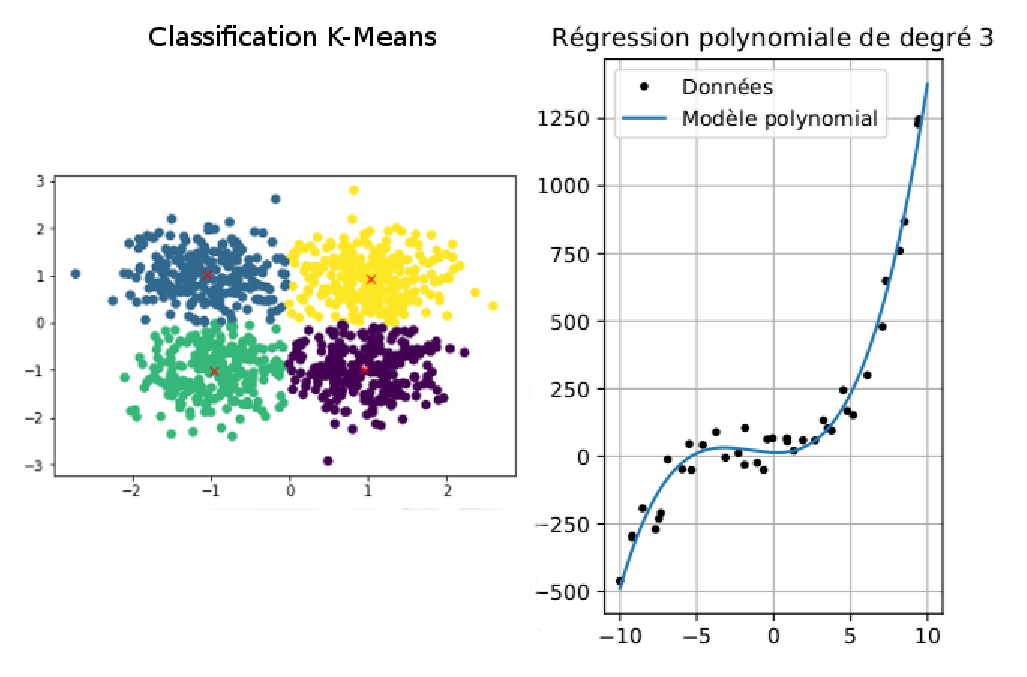
\includegraphics[scale = 0.8]{annex/ex_mach_lr}
				\caption{Exemple de méthodes de Machine Learning}
				\label{example}
			\end{center}
		\end{figure}\p

		Dans le cadre de mon stage, je me suis plus intéressé aux méthodes de Deep Learning\index{Machine Learning!Deep Learning} qui s'avèrent être un cas particulier de Machine Learning. Il s'agit de méthodes utilisant des réseaux de neurones\index{Machine Learning!Deep Learning!neural networks}. Un réseau de neurones\index{Machine Learning!Deep Learning!neural networks} est composé de plusieurs couches et chaque couche est composée de plusieurs ``neurones''. Dans le cas des réseaux de neurones\index{Machine Learning!Deep Learning!neural networks} un ``neurone'' représente une opération élémentaire comme une addition ou une multiplication. Cette succession d'opération élémentaires permet de réaliser des modèle mathématiques plus développé et ainsi d'apprendre ``plus en profondeur'' comment s'agence les données. C'est de ce principe que vient le terme de Deep Learning.\p

		Les méthodes de Deep Learning\index{Machine Learning!Deep Learning} epuvent aussi se décomposer en plusieurs groupes. Parmi ceux ci se trouve la segmentation, qui est la méthode que j'ai étudié au cours de ce stage. La segmentation\index{Machine Learning!Deep Learning!segmentation} est le principe de déterminer au sein d'un élément d'un jeu de données, une image par exemple, différentes classes. Ces méthodes sont différentes des méthodes de classification\index{Machine Learning!classification} qui consiste à classer les éléments du jeu de données.\clearpage
		\begin{figure}
			\begin{center}
				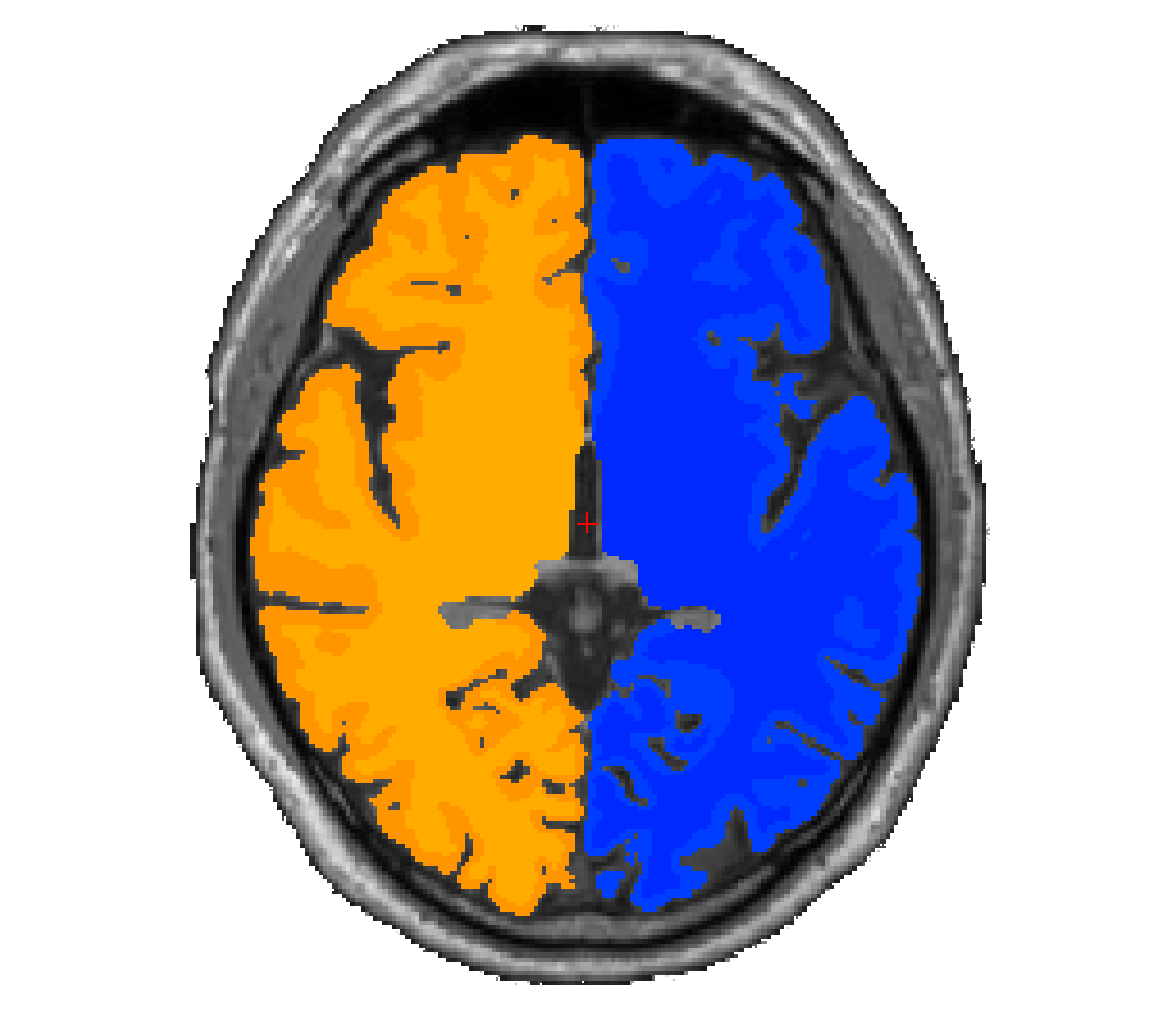
\includegraphics[scale=0.5]{annex/segmentation}
				\caption{exemple de segmentation}
				\label{segmentation}
			\end{center}
		\end{figure}\p

		Actuellement, les techniques de Machine Learning\index{Machine Learning} et de Deep Learning\index{Machine Learning!Deep Learning} sont de plus en plus utilisées, notamment dans le domaine médical permettant ainsi de faciliter la tâche des médecins lors de l'analyse d'IRM\index{IRM} par exemple. Il est donc important que les méthodes utilisées soient fiables, mais cela pose aussi problème si l'ordinateur met plus de temps que l'humain pour déterminer la présence de tumeur. Mon travail a donc été de déterminer une méthode pour diminuer le temps d'apprentissage du modèle pour une méthode de segmentation\index{Machine Learning!Deep Learning!segmentation}.\p

	\chapter{Contexte}

		Les méthodes de prédiction de Deep Learning ont connu un certain essort dans tous les domaines. Ainsi, un certain nombre de librairies (Python\index{Python}) open-source\index{open-source} permettant de réaliser des réseaux de neurones\index{Machine Learning!Deep Learning!neural networks} ont vu le jour comme TensorFlow\index{Python!TensorFlow} ou encore FastAI.\p

		\section{NiftyNet}

		Pour faciliter un usage plus spécifique de la librairie TensorFlow\index{Python!TensorFlow}, la plate-forme NiftyNet\index{NiftyNet} a vu le jour. Cette plate-forme open-source\index{open-source} s'est spécialisée dans le domaine médicale et dans la lecture des images issues des IRM\index{IRM}. Cette plate-forme permet une fois installée de réaliser des réseaux de neurones\index{Machine Learning!Deep Learning!neural networks} sans avoir une très grande connaissance du langage de programmation, seule la complétion du fichier de configuration est nécessaire au bon fonctionnement du réseau.\p

	\chapter{Méthodes}

	\chapter{Difficultés rencontrées}

	\chapter{Résultats}

	\backmatter

	% \newglossaryentry{alti}{
	%   name={Altipharma},
	%   plural={Altipharma},
	%   description={groupe de pharmacies}
	% }

	\clearpage
	\addcontentsline{toc}{chapter}{Index}
	\printindex

	% \printglossary
	% \addcontentsline{toc}{chapter}{Glossaire}

	\nocite{*}
	\bibliographystyle{plain}
	\bibliography{annex/biblio_stage}
	\addcontentsline{toc}{chapter}{Bibliographie}

\end{document}
